
\chapter{Discussion}

\acresetall


\section{Humanly Perceived Improvement vs. Machine Performance}

The aim of conducting research into existing data was to determine,
at a basic level, the correlation between \ac{HR} and \ac{MR}.


\subsection{Investigating Existing Data}

Results from conducting a direct comparison between \ac{PESQ} and
\ac{PRR} results were given in \figref{Direct-PESQ-PRR}. These results
show a general, positive correlation between \ac{PESQ} improvement
and \ac{PRR} improvement, and by extension between \ac{HR} and \ac{MR}.
The level of correlation appears to be relatively low, however comparison
with \figref{litResCorr} indicates the such levels of correlation
are expected. Indeed, similar correlations are observed between \ac{PESQ}
and \ac{MOS} results, which are both \ac{HR} measures.

\figref{litResCorr} Also indicates a very high correlation between
the raw \ac{PESQ} result and \ac{PRR}.

A number of further observations were drawn from \figref{Direct-PESQ-PRR},
and are highlighted in \Cref{fig:direct-klt-mband,fig:direct-klt-pklt,fig:direct-pklt-logmmse-spu-4,fig:direct-highcorr}.

Despite the high correlation between \ac{PESQ} and \ac{PRR} observed,
there is still evidence to show that algorithms' performances vary
depending on the performance measure used. For example, highlighted
in \figref{direct-klt-mband} are two algorithms, the \ac{KLT} method
and the \ac{MBAND} method, that exhibited similar performances when
evaluated by \ac{PRR}, a machine measure. However, when evaluated
by a human perceptual method, \ac{PESQ}, the \ac{KLT} method clearly
performed better. In fact, the \ac{KLT} method exhibited one of the
best performances seen on the \ac{PESQ} scale, whereas the \ac{MBAND}
method was the worst performer on this scale, exhibiting loss in perceptual
quality, as indicated by the negative performance.

\begin{figure}[h]
\noindent \begin{centering}
\includegraphics[width=0.8\textwidth]{fig/R/dir/lit/KLT-MBAND/HumanMachineAllLM}\includegraphics[width=0.2\textwidth]{fig/R/dir/lit/HumanMachineAllLegend}
\par\end{centering}

\protect\caption{\label{fig:direct-klt-mband}Direct comparison of \acs{PESQ} vs.
\acs{PRR} highlighting \acs{KLT} and \acs{MBAND}}
\end{figure}


\figref{direct-klt-pklt} shows the \ac{PESQ} vs. \ac{PRR} improvement
with the \ac{KLT} and \ac{pKLT} algorithm performances highlighted.
This was noted as an example of two very similar algorithms, with
varying performance between \ac{HR} and \ac{MR} results. The \ac{KLT}
results exhibited better performance for a human listener, as the
points laid higher on the y-axis, whereas the \ac{pKLT} results exhibited
better performance for a machine recogniser, as the points laid higher
on the x-axis.

\begin{figure}[p]
\noindent \begin{centering}
\includegraphics[width=0.8\textwidth,height=0.25\textheight,keepaspectratio]{fig/R/dir/lit/KLT-pKLT/HumanMachineAllLM}\includegraphics[width=0.2\textwidth,height=0.25\textheight,keepaspectratio]{fig/R/dir/lit/HumanMachineAllLegend}
\par\end{centering}

\protect\caption{\label{fig:direct-klt-pklt}Direct comparison of \acs{PESQ} vs. \acs{PRR}
highlighting \acs{KLT} and \acs{pKLT}}
\end{figure}


Such results support the proposition that some algorithms are inherently
suited either towards human or machine listeners. However, this shows
that such distinction is not necessarily related to the algorithm
class, since the \ac{KLT} and \ac{pKLT} algorithms belonged to the
same \ac{KLT} class, but produced different results.

The \ac{pKLT} and \ac{logMMSE-SPU-4} algorithms were observed to
show reasonable improvement in \ac{PRR} as the \ac{SNR} increased,
but little to no improvement in \ac{PESQ}. This is highlighted in
\figref{direct-pklt-logmmse-spu-4}, and is apparent by the near-zero
gradient. These algorithms likely introduce distortions into the signal
in the process of enhancement that the \ac{ASR} algorithm was immune
to, however would be distracting to a human and therefore performed
badly under the \ac{PESQ} evaluation.

\begin{figure}[p]
\noindent \begin{centering}
\includegraphics[width=0.8\textwidth,height=0.25\textheight,keepaspectratio]{fig/R/dir/lit/pKLT-logMMSE-SPU-4/HumanMachineAllLM}
\par\end{centering}

\protect\caption{\label{fig:direct-pklt-logmmse-spu-4}Direct comparison of \acs{PESQ}
vs. \acs{PRR} highlighting \acs{logMMSE} \acs{SPU} and \acs{pKLT}}
\end{figure}


The final observation drawn from \figref{Direct-PESQ-PRR} is highlighted
in \figref{direct-highcorr}, which shows the \ac{MMSE-SPU}, \ac{STSA-wcosh},
\ac{STSA-weuclid} and \ac{logMMSE-SPU-3} algorithms. These algorithms
show a high, positive correlation with one another, as well as exhibiting
the best results measured for both \ac{PESQ} and \ac{PRR}. The evidence
suggests such a response is the ideal case, and that there exists
algorithms which are capable of performing well for both human and
machine recognisers.

\begin{figure}[p]
\noindent \begin{centering}
\includegraphics[width=0.8\textwidth,height=0.25\textheight,keepaspectratio]{fig/R/dir/lit/MMSE-SPU-STSA-wcosh-STSA-weuclid-logMMSE-SPU-3/HumanMachineAllLM}
\par\end{centering}

\protect\caption{\label{fig:direct-highcorr}\acs{STSA-wcosh}, \acs{STSA-weuclid}
and \acs{logMMSE-SPU-3}}
\end{figure}


Results found using the grouped comparison method, shown in \figref{Group-PESQ-PRR-LOESS}
indicated that the data could be approximated by a linear model. The
\ac{LOESS} fitted lines were, in most cases, approximately linear.
The results for Wiener algorithms were a notable exception, with a
non-linear variation, even when the outliers are ignored. Overall,
the \ac{LM} fit in \figref{Group-PESQ-PRR-LM} is accepted to be
accurate.

The grouped linear fittings also correlate well with the best performing
individual algorithms, those highlighted in \figref{direct-highcorr}.


\subsection{Independent Investigation into \acl{HR} and \acl{MR}}

An independent investigation was conducted in which a number of enhancement
algorithms were implemented. The enhanced waveforms were then analysed
using a number of enhancement methods, covering both \ac{HR} and
\ac{MR}. The goal was to determine the correlation between evaluation
measures.

A summary of the correlation between all measurements made is given
in \figref{my-Corr}. A number of interesting observations were drawn
from this summary to be further investigated.


\subsubsection*{On the relationship between \acs{PESQ} and \acs{MOS}}

Firstly, it was noted that in \figref{my-Corr}, the correlation between
\ac{PESQ} and the various \ac{MOS} measures was low. This was a
surprising results as it has generally been determined in literature
that the two correlate well \cite{Kitawaki2007,Rix2003,Rix2001},
albeit with some exceptions \cite{Liu2006}. It was also noted that
the ideal binary mask algorithms performed very poorly overall on
the subjective scales in \Cref{fig:my-MOS,fig:my-MOSle,fig:my-CMOS}.
Furthermore, ideal binary mask algorithms had a very high variation
in \ac{PESQ} performance in \figref{my-PESQ}. Therefore, it was
suspected these results may be adversely affecting the overall correlation
between \ac{PESQ} and \ac{MOS}.

It was found that when the ideal binary mask algorithm data was omitted
the correlation between the \ac{PESQ} and \ac{MOS} increased, as
demonstrated in \figref{my-pesq-mos}. This indicated there were specific
occurrences for which the relationship between \ac{PESQ} and \ac{MOS}
demonstrated in literature do not hold. 

\begin{figure}[h]
\subfloat[With the ideal binary mask]{

\includegraphics[width=0.5\textwidth]{fig/R/pair/my/pesq-mos}

}\subfloat[Without the ideal binary mask]{

\includegraphics[width=0.5\textwidth]{fig/R/pair/my/pesq-mos_no-IDBM}

}

\includegraphics[width=1\textwidth]{fig/R/pair/my/pesq-mos_leg}

\protect\caption{\label{fig:my-pesq-mos}Scatterplot of \acs{PESQ} vs. \acs{MOS}
results}
\end{figure}



\subsubsection*{On the relationship between similar measures}

The \ac{MOS} evaluation measures had a strong correlation with one-another
in \figref{my-Corr}, all at approximately 90\%. This was expected
between similar measures. However, it was noted that the same was
not true for the \ac{PRR} measures, where the correlation between
the correctness and the accuracy was found to be in general significantly
negative.


\subsubsection*{On the relationship between \acl{HR} and \acl{MR}}

\figref{my-Corr} shows a significant positive correlation between
the various \ac{MOS} measures and the \ac{PRR} measured as correctness.
However, the figure also shows an almost as significant negative correlation
between the various \ac{MOS} measures and the \ac{PRR} measured
as accuracy. \Cref{fig:mos-prrcorr,fig:cmos-prrcorrimp} highlight
the correlation between \ac{MOS} and \ac{PRR} measured as correctness.
\figref{mos-prrcorr} further highlights the relative density, revealing
that certain test conditions are outliers and that the correlation
might otherwise have been higher. It was seen that tests where there
was one competing speaker of the same sex, highlighted in red, were
characterised by a mid-range \ac{MOS} result, but a high correctness
\ac{PRR}. This indicated the \ac{ASR} system was able to still detect
the \ac{SoI}'s voice, however a human listener scored the signal
as average.

However, \figref{cmos-prraccimp} shows that in terms of improvement,
and regardless of algorithm, the enhancement in competing speaker
noise was non-existent. NOIZEUS babble noise results tended also to
be poor. Interestingly, the synthetic babble formed from three speakers
tended to be improved by most algorithms under the accuracy \ac{PRR}
measure. This had almost no correlation with the performance rated
by human listeners, which ranged from a fair improvement to significantly
worse.

\begin{figure}[h]
\subfloat[\label{fig:mos-prrcorr}\acs{MOS} vs. \acs{ASR} correctness]{\includegraphics[width=0.5\textwidth]{fig/R/pair/byTest/mos-prrcorr}

}\subfloat[\label{fig:mos-prracc}\acs{MOS} vs. \acs{ASR} accuracy]{\includegraphics[width=0.5\textwidth]{fig/R/pair/byTest/mos-prracc}

}

\subfloat[\label{fig:cmos-prrcorrimp}Comparative \acs{MOS} vs. \acs{ASR}
correctness improvement]{\includegraphics[width=0.5\textwidth]{fig/R/pair/byTest/cmos-prrcorrimp}

}\subfloat[\label{fig:cmos-prraccimp}Comparative \acs{MOS} vs. \acs{ASR} accuracy
improvement]{\includegraphics[width=0.5\textwidth]{fig/R/pair/byTest/cmos-prraccimp}

}

\noindent \begin{centering}
\includegraphics[width=0.6\linewidth]{fig/R/pair/byTest/mos-prr-leg}
\par\end{centering}

\protect\caption{\label{fig:hr-mr}Scatterplot of \acs{HR} and \acs{MR} measures,
highlighting test conditions}
\end{figure}


\figref{hr-mr-alg} shows the same data as \figref{hr-mr}, but with
colour highlighting the enhancement algorithm as opposed to the test
conditions. A very interesting observation made was the performance
of the ideal binary mask and phoneme-dependent ideal binary mask,
especially under accuracy \ac{PRR}. These results were also noted
by observing the ideal binary mask algorithms performance in \Cref{fig:my-PRRacc,fig:my-PRRacc-imp}.
These algorithms achieved the highest scores of any algorithm, despite
performing poorly on all \ac{HR} and statistical measures.

The explanation given for this behaviour was that the ideal binary
mask algorithms are effective in eliminating the competing noise,
and thus reducing false insertions. However, in the process these
algorithms distort the signal severely, thereby drastically reducing
human intelligibility, and also causing the loss in correctness \ac{PRR}
exhibited in \figref{my-PRRcorr-imp}. 

\begin{figure}[h]
\subfloat[\label{fig:cmos-prrcorrimp-alg}Comparative \acs{MOS} vs. \acs{ASR}
correctness improvement]{\includegraphics[width=0.5\textwidth]{fig/R/pair/byAlg/cmos-prrcorrimp}

}\subfloat[\label{fig:cmos-prraccimp-alg}Comparative \acs{MOS} vs. \acs{ASR}
accuracy improvement]{\includegraphics[width=0.5\textwidth]{fig/R/pair/byAlg/cmos-prraccimp}

}

\noindent \begin{centering}
\includegraphics[width=0.9\linewidth]{fig/R/pair/byAlg/mos-prr-leg}
\par\end{centering}

\protect\caption{\label{fig:hr-mr-alg}Scatterplot of \acs{HR} and \acs{MR} measures,
highlighting enhancement algorithm}
\end{figure}


\clearpage{}


\section{Assessing \acl{NMF} Algorithm Training}


\subsection{Investigating Training Requirements}

The investigation to investigate training was conducted on two recently
proposed \ac{NMF} algorithms of interest, an online \ac{BNMF} and
a supervised \ac{BNMF}.


\subsubsection*{General Performance}

The algorithm performance was poor on the supplied test data. It can
be seen in \figref{vary-train-pesq-imp} that in general the enhanced
algorithm performed worse than the dirty recording, by the fact that
the improvement scores are predominantly negative. The algorithms
produced similar patterns consistently across tests, indicating it
is unlikely results are randomised outliers.


\subsubsection*{Online \acl{BNMF}}

Before tests were performed, it was hypothesised that increasing the
number of utterances provided as training would allow the algorithm
to produce a better model, with more data to learn from. However,
the number of utterances provided for training of the online \ac{BNMF}
algorithm in \figref{vary-train-pesq} had no significant impact on
\ac{PESQ} performance. In fact, a slight negative correlation may
be noted, which is supported by results in \figref{train-req-corr}.

\clearpage{}


\section{Phoneme-Dependent Variation Performance}

\figref{drawn-phoneme-spectrogram} shows a typical example of the
drawn phonemes that were used for training data. The differences in
phonemes is clear and identifiable, indicating that the method worked
as intended. One issue noted was that voiceless stops, were too short
and were occasionally missed. An example is noted in the first two
phoneme samples in \figref{mos-comparison-phn-1}, which are /p/ and
/t/. For such phonemes, high frequency components would have been
expected, but were not present. The same phonemes in \figref{mos-comparison-phn-5}
revealed that only 2 out of the 10 phoneme slices contained the expected
high frequency components. However, these kind of errors were expected
and is one of the reasons that the number of slices per phoneme was
varied.

Also noted was the fact that there was little to no visual difference
after 50 to 100 phoneme samples were drawn. Additionally noted was
the fact that the length of recordings stopped increasing around this
point. After this point the saturation point for the recordings used
was reached, where there were not enough phoneme occurrences to support
having more samples. So the tests done for more samples per phoneme
than 100 were redundant.


\subsection{Performance for Humans}

\figref{pesq-comparison-phn} indicated that the phoneme dependent
\textbf{training} modifications caused, in general, a decline in performance
measured with \ac{PESQ}. The opposite was true, however, for the
phoneme \textbf{base} modification algorithms. These algorithms mostly
scored higher, with the exceptions mostly belonging the the NOIZEUS
street noise tests.

This is in contrast, however, to the \ac{MOS} results presented in
\Cref{fig:mos-comparison-phn,fig:mosle-comparison-phn,fig:cmos-comparison-phn}.
These results did not show any specific pattern of improvement across
different noise types. This indicated that the phoneme dependence
modifications to these algorithms did not present any significant
improvement for human listeners.

It was noted, however, that the points that did show better enhancement
on the \ac{MOS} scales were more likely to be of the synthetic babble
noise types, c3f(m) and c3f(m)+c3c(f)+c35(m). These are also associated
with the more ``difficult'' forms of noise. Therefore, it is possible
that using phoneme dependence in algorithms may be useful in source
separation applications. This highlights the ability of phoneme dependence
to distinguish between voices, but not as an efficient method of extracting
speech from other noise.


\subsection{Performance for Machines}

The phoneme-dependent \textbf{training} modifications failed to improve
machine correctness almost completely, as indicated in \Cref{fig:prrcorr-comparison-phn,fig:prrcorrimp-comparison-phn}.
However, with the exception of the ideal binary mask algorithms and
the c3f(m) noise type, the phoneme-dependent \textbf{training} modifications
tended to improve the machine correctness. This suggests that using
phoneme dependence tends to both increase the algorithm's ability
to remove noise, but also increases the distortion. This observation
makes sense, as using phoneme-dependent \textbf{training} is in some
ways a means to prevent over-training, so some under-trained characteristics
like this were to be expected.

Interestingly, the increased correctness suggests that the noise reduction
outweighs the distortion for a machine recogniser. The poor performance
for the c3f(m) noise type is attributed to the fact that both the\ac{SoI}
and the noise are a similar male voice. The poor performance indicated
that phoneme-dependent \textbf{training} did not particularly aid
in separating similar voices. The poor accuracy was likely due to
a high number of false positive phoneme detections, detected from
the second voice.

The phoneme-dependent \textbf{base} modifications showed improvement
in correctness, unlike the phoneme-dependent \textbf{training} modifications,
as best observed in \figref{prrcorr-comparison-phn}. However, in
terms of accuracy, no significant pattern was noted between those
performing better and worse than the original algorithms.


\subsection{Other Observations}

The performance for the \ac{MMSE} algorithm is unchanged by the introduction
of phoneme-dependence across the objective measures. This indicated
that using phoneme dependence did not affect the operation of this
particular algorithm. This also highlighted the level of subjectivity
involved in the \ac{MOS} tests, since the scores for the \ac{MMSE}
algorithm in \Cref{fig:mos-comparison-phn,fig:mosle-comparison-phn,fig:cmos-comparison-phn}
deviated quite significantly from the diagonal line.
